\documentclass[10pt,a4paper]{scrartcl}
\usepackage[utf8]{inputenc}
\usepackage[ngerman]{babel}
\usepackage{amsmath}
\usepackage{amsfonts}
\usepackage{amssymb}
\usepackage{marvosym}
%\usepackage{gensymb}
\usepackage{graphicx}
\usepackage{hyperref}
\usepackage{url}
\usepackage{siunitx}
\usepackage{bookmark}
\sisetup{locale = DE}

\renewcommand{\UrlFont}{\small\tt}
\usepackage[a4paper,lmargin={2.5cm},rmargin={2.5cm},tmargin={2.5cm},bmargin = {2.5cm}]{geometry}

\linespread{1.1}

\begin{document}

\pagenumbering{Roman}

\title{SALOME\\Simple Accelerator for Learning Optics and
Manipulation of Electrons}
\subtitle{Fortgeschrittenenpraktikum\\ Versuch EXP9}
\author{Léonie Lanz \\ Nico Kalogerakis}
\maketitle
\newpage

\tableofcontents
\vfill
\newpage

\pagenumbering{arabic}

\section{Einleitung}

\section{Theoretische Grundlagen}
\subsection{Dipol}

\subsection{Quadrupol}

\subsection{Betatron-Strahlung und Emittanz}

\section{Experimenteller Aufbau}

\section{Versuchsdurchführung}
Messmethoden:\\
how emittanz\\
quadrupolscan (nur mit matrizenformalismus)\\
how energie\\
strahlbasierte justage\\
Strahltransport

\section{Auswertung der Messergebnisse}

\subsection{Strahltransport}
Bilder

\subsection{Strahlbasierte Justage}
\subsubsection{x Werte}
$I_{Q_{1}} = -0.344$ plot\\
$I_{Q_{2}} = 0.657$ plot\\
$I_{D_{0}} = -1.236$ (x intersection) 

\begin{figure}[ht!]
    \centering
    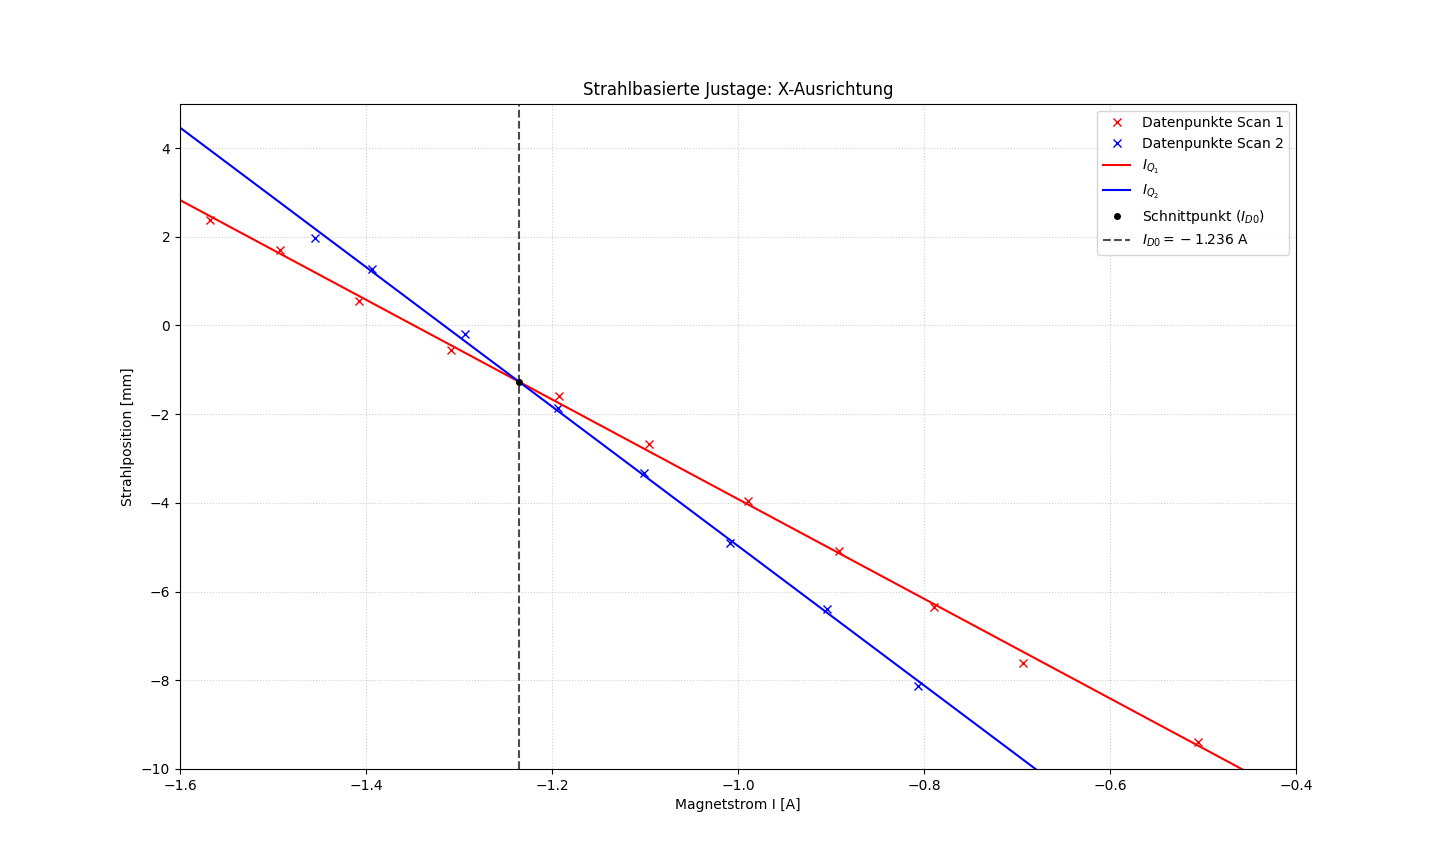
\includegraphics[scale=0.435]{img/Strahlbasierte Justage_X-Ausrichtung.png}
    \caption{Strahlbasierte Justage in x-Ausrichtung}
\end{figure}

\subsubsection{y Werte}
$I_{Q_{1}} = 1.685$ plot \\
$I_{Q_{2}} = 2.703$ plot \\
$I_{D_{0}} = -0.777$ (y intersection) plot

\begin{figure}[ht!]
    \centering
    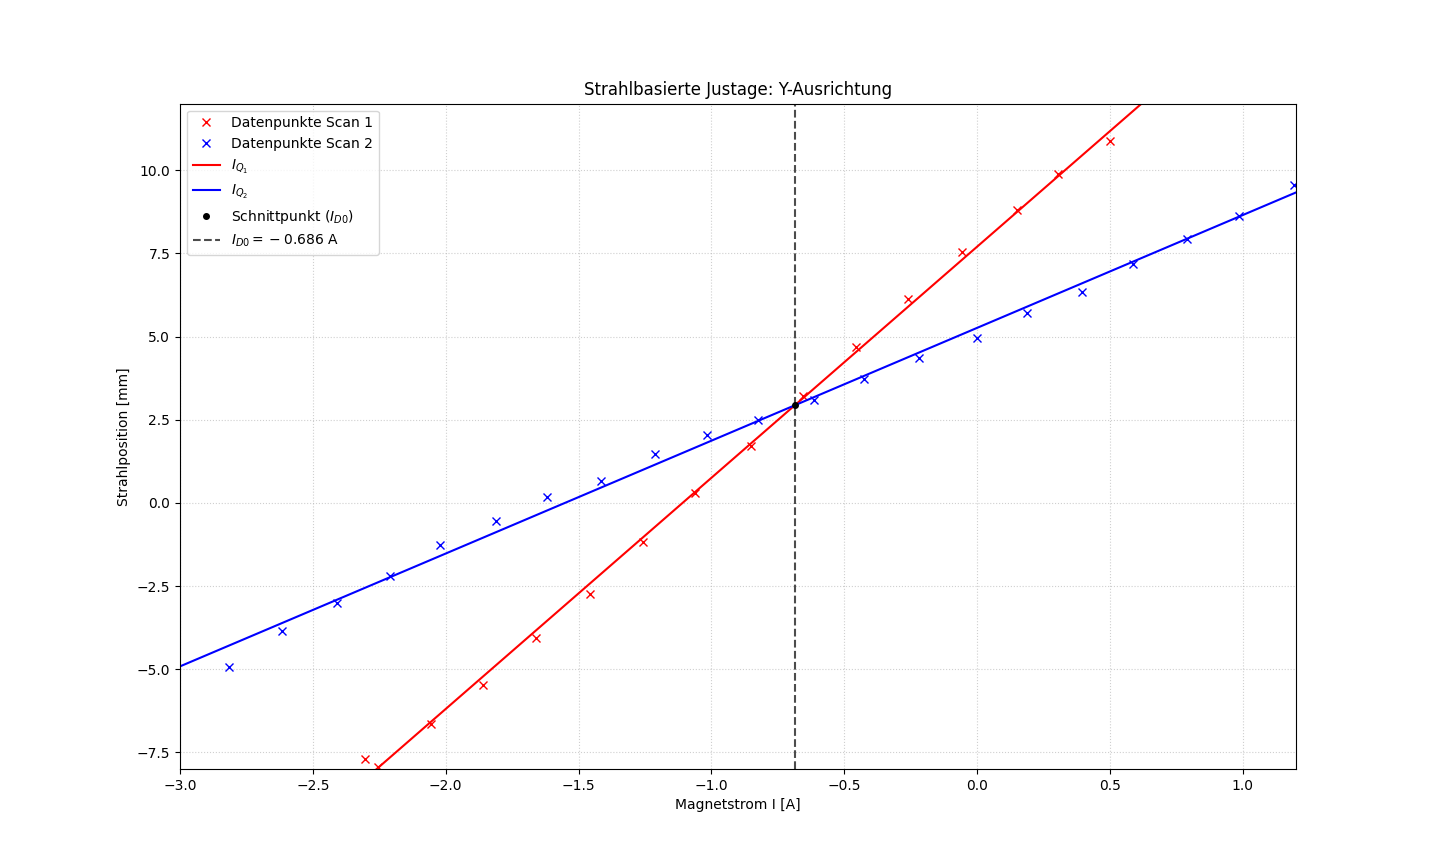
\includegraphics[scale=0.435]{img/Strahlbasierte Justage_Y-Ausrichtung.png}
    \caption{Strahlbasierte Justage in y-Ausrichtung}
\end{figure}

\subsubsection{Fehler}
Mittlerer Scanschritt x = 0.1063
Fehler x: $\frac{\Delta_I}{2} = 0.0532$

Mittlerer Scanschritt y = 0.1869
Fehler y: $\frac{\Delta_I}{2} = 0.0935$

\begin{figure}[ht!]
    \centering
    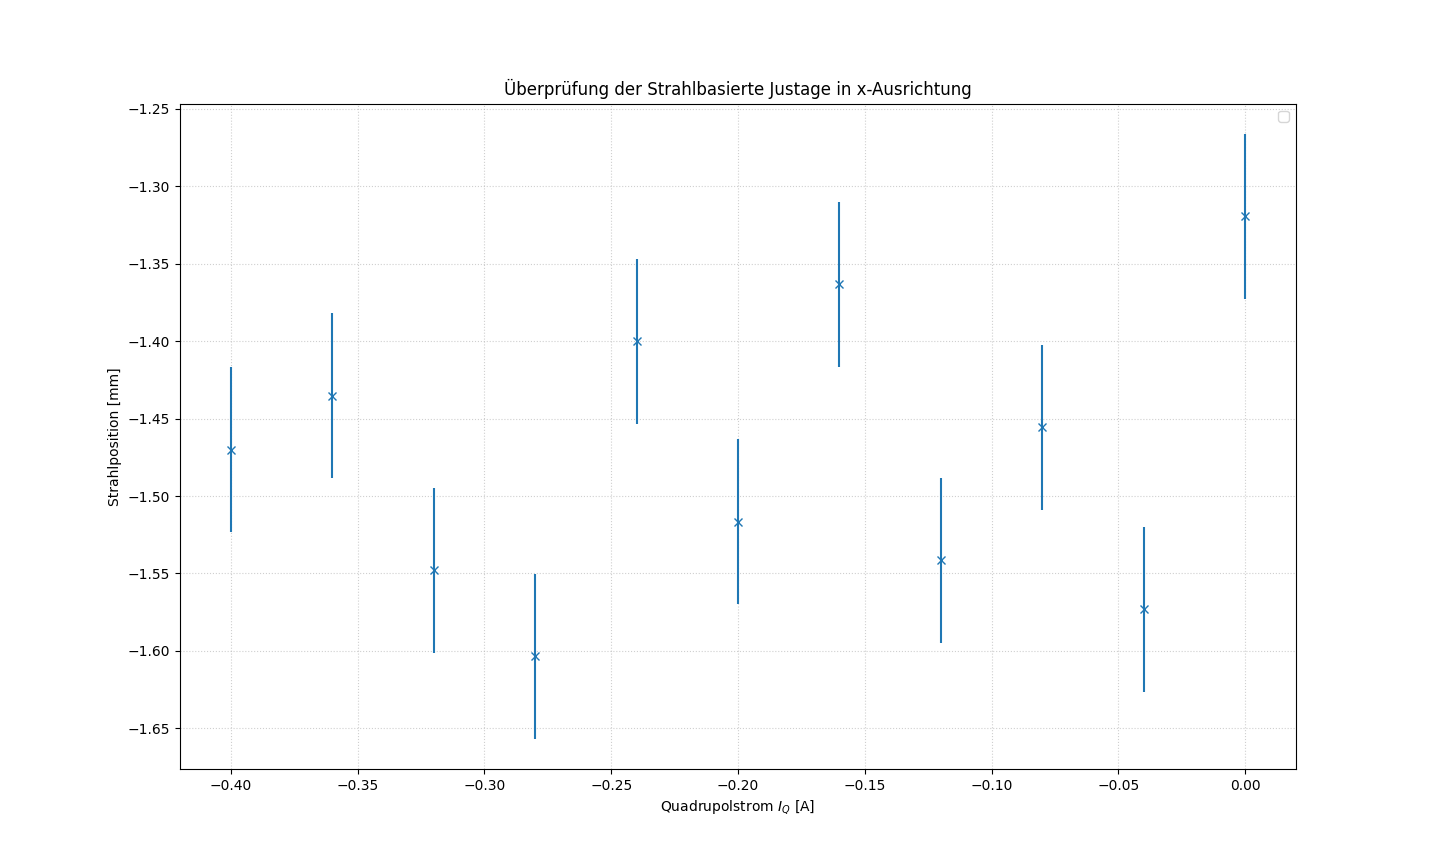
\includegraphics[scale=0.435]{img/Überprüfung der Strahlbasierte Justage_x.png}
    \caption{Überprüfung der Strahlbasierte Justage in x-Ausrichtung}
\end{figure}

\begin{figure}[ht!]
    \centering
    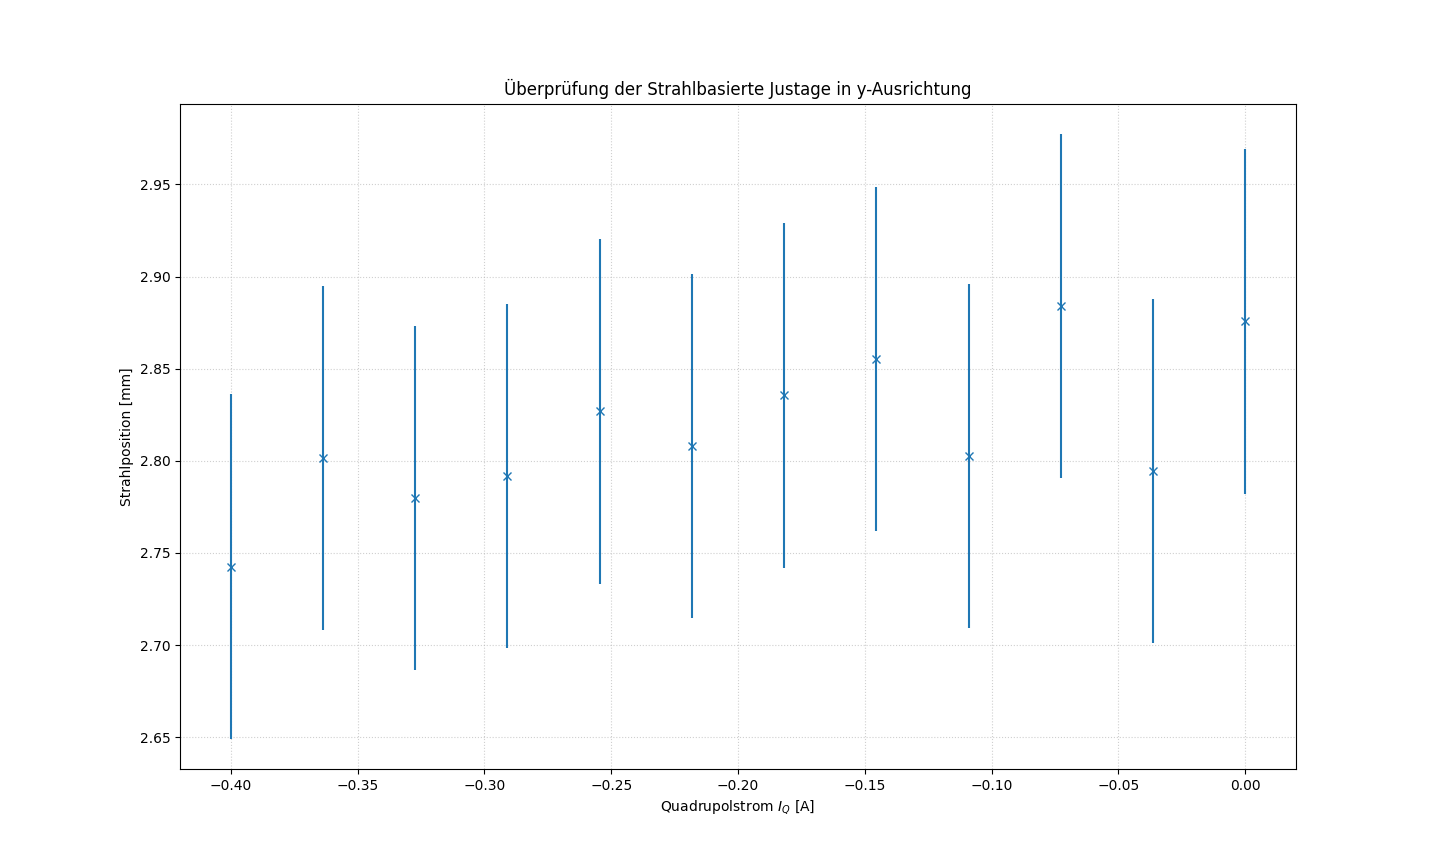
\includegraphics[scale=0.435]{img/Überprüfung der Strahlbasierte Justage_y.png}
    \caption{Überprüfung der Strahlbasierte Justage in y-Ausrichtung}
\end{figure}

\subsection{Energiemessung}
\begin{math}
\frac{dy}{dI} = 14.4384 \frac{mm}{A} \pm 0.106 \frac{mm}{A}\\
\kappa = 7.64 \cdot 10^{-6} \frac{Tm}{A}\\
L = 0.52 m \pm 0.01 m\\
E_0 = 511 keV\\
\beta \gamma = 0.1614 \pm 0.00332 \approx \beta\\
\gamma = 1.013 \pm 0.000529 \rightarrow \text{ also fast klassisch}\\
E_{kin} =6.62 keV \pm 0.27 keV\\
p = 2.752 \cdot 10^{-7} \frac{keV}{c} \pm 5.661 \cdot 10^{-9} \frac{keV}{c}\\
\end{math}

\subsection{Emittanz}

$\epsilon_x = 0.72867 \pm 0.07115$ mm mrad\\
$\epsilon_y = 1.98349 \pm 0.09011$ mm mrad

\subsubsection{Optische Funktionen}

$\beta_x = 0.578 \pm 0.0565, \alpha_x = -1.19 \pm 0.117, \gamma_x = 4.19 \pm 0.41$\\
$\beta_y = 0.814 \pm 0.037, \alpha_y = -1.401 \pm 0.0637, \gamma_y = 3.639 \pm 0.165$

\subsection{Beta-Func}

\begin{figure}[ht!]
    \centering
    
\includegraphics[scale=0.435]{img/beta func mit fehlerfortpflanzung.png}
    \caption{$\beta$-Funktion in Abhängigkeit der z-Position des Strahls}
\end{figure}

\section{Diskussion der physikalischen Ergebnisse}


\section{Zusammenfassung}


\newpage

\pagenumbering{Alph}

\bibliography{literatur.bib}
\addcontentsline{toc}{section}{Literatur}

\newpage

\listoffigures 
\addcontentsline{toc}{section}{Abbildungsverzeichnis}

\end{document} 